\documentclass[12pt]{article}
\usepackage{graphicx}
\begin{document}
\begin{center}
  {\large\bf Track Reconstruction and Vertex Finding}
\end{center}
\vskip0.2in
Goals:
\begin{itemize}
\item Introduce the concept of track fitting using the example of a straight line
  fit
\item Understand the meaning of track impact parameter  and calculate the
  dependence of impact parameter resolution on the relevant detector parameters
\item Use Monte Carlo techniques to demonstrate that the decay products of
  long-lived particles can  be ``tagged'' by selecting tracks with high
  impact parameter
\item Use the example of a simple two-body decay to introduce the topic of
  secondary vertex reconstruction.
\end{itemize}
Silicon microstrip and pixel detectors play a prominent role in many particle
physics experiments.  Their good spatial resolution, ability to distinguish
near-by particles and radiation hardness make them attractive options.  You
have studied the position resolution of such detectors in a previous homework.
Today, we will learn about how they are used to reconstruct particle trajectories
and to identify the decay products of weakly decaying particles.

Track reconstruction is performed in several steps.  First, neighboring hits are
combined to form space-points.  Second, a pattern recognition
algorithm is used to associate a set of space-points with a single trajectory.
Finally, these space-points are fit to determine track parameters.  This problem
focuses on the final stage where track parameters are determined.

In this problem
we will consider the case of a charged particle traversing multiple silicon
  strip detectors leaving a straight line trajectory.  An example
  of this case is the LHCb VErtex LOcator (VELO) detector.  See\\
  https://lhcb-public.web.cern.ch/lhcb-public/en/detector/VELO2-en.html\\
  In addition, while the ATLAS and CMS trackers are placed in a solenoidal
  magnetic field, fits in the non-bending plane ($r$-$z$ in cylindrical
  coordinates with the $B$ field along the $z$-axis) will be straight lines.
\newpage
\begin{enumerate}
\item {\it Track Fitting from Silicon Space Points}
\begin{center}
  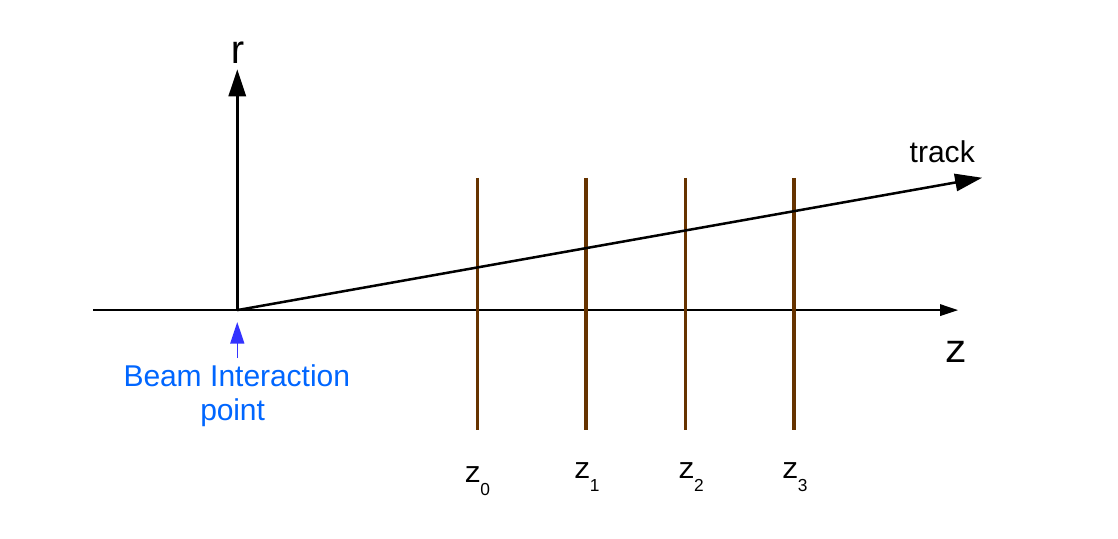
\includegraphics[width=4.0in]{tracker.png}
\end{center}  Consider a very simplified model of a tracking
  detector.  The detector will consist of 4 layers of silicon equally spaced
  with the first layer a distance $z_0$ from the beam interaction point and a
  $z$-spacing  between layers of $\ell$.
  The $z$ position of the detectors is perfectly
  known.  The strips are oriented to give a measurement of $r$ in each detector
  with a resolution $\sigma_r$.
  The track is a straight line, so it can be described as
  trajectory in the $r$-$z$ plane
  $$
    r = az + b 
  $$
  where the best estimates of $a$ and $b$ are obtained using a $\chi^2$ fit
  to the 4 spacepoints.
  \begin{enumerate}
  \item If $r_0$ through $r_3$ are the measured hit positions on
    the 4 layers of silicon, find analytic expressions for the fit
    values of $a$ and $b$. Express your answer in terms of the $z$ positions
    of the sensors and the measured $r$ positions.  
  \item Find an expression for the uncertainty on the intercept $b$.
  \item Generate 1000 tracks all coming from the
    beam interaction point (these are called ``primary tracks'')
    and distributed uniformly in $\cos\theta$ for
    $-0.25 < \theta < 0.25$.  For each track, simulate the measured hit positions
    using a resolution $\sigma_r=15\;\mu$m and fit the measured
    hits to determine $m$ and $b$.  Use the values $z_0=5$~cm and $\ell=10$~cm.
    Make a histogram of the fit values of $b$ for the tracks and
    verify that the width of the distribution agrees with your analytic result above.
  \item The track impact parameter $d_0$ is defined as the distance of closest
    approach of the track to the the beam interaction point.  For
    a track with trajectory $r = az +b$, find an expression for $d_0$.
  \item Consider the case of a $B^0$ meson
    (mass=$5.28$~GeV, lifetime=$1.52\times 10^{-12}$~s) with a momentum of 25~GeV.
    On average, such mesons will travel about 2000~$\mu$m before decaying.  Their
    decay products therefore will not intersect the beam interaction point.
    We will study the rare decay $B^0\rightarrow \pi^+ \pi^-$.  Generate 1000
    primary $B^0$ mesons and allow them to decay according to the normal
    exponential decay formula. For cases
    where both tracks are produced with $-0.25 < \theta < 0.25$, find the
    fitted values of $b$ and $m$ for each track and make a histogram of
    the value of $d_0$. (Note: the
    two body decay is isotropic in the $B^0$ center of mass).
    Compare (using a log scale for your $y$-axis) the
    $d_0$ distribution of the $B^0$ decay products to those of primary tracks.
    Explain how you would select a sample of events enriched in $B$ meson decays.
  \item An even better technique for identifying long-lived particles is to
    reconstruct a secondary vertex from tracks with large impact parameter.
    For the $B^0$ sample generated above, find the position where the two
    tracks cross and make a histogram of the distance of the decay from the
    beam interaction point.
    Generate a sample where each event contains two primary tracks
    and compare the decay distance distributions of the two samples.
  \end{enumerate}
\end{enumerate}
\end{document}
